\documentclass{beamer}
\usepackage[edges]{forest}
\usepackage{tikz}
\usepackage{media9}
\usetikzlibrary{arrows.meta, positioning, shapes.geometric}
\usepackage{graphicx}
\usepackage[utf8]{inputenc}
\usepackage[T1]{fontenc}
\usepackage[style=authoryear, backend=biber]{biblatex}
\usepackage{listings}
\usepackage{xcolor}
\usepackage{pdfpages}
\usepackage{amsmath}
\usepackage{amsfonts}
\addbibresource{main.bib}

\definecolor{mGreen}{rgb}{0,0.6,0}
\definecolor{mGray}{rgb}{0.5,0.5,0.5}
\definecolor{mPurple}{rgb}{0.58,0,0.82}
\definecolor{backgroundColour}{rgb}{0.95,0.95,0.92}

\lstdefinestyle{CStyle}{
    basicstyle=\ttfamily\tiny,
    backgroundcolor=\color{backgroundColour},   
    commentstyle=\color{mGreen},
    keywordstyle=\color{magenta},
    numberstyle=\tiny\color{mGray},
    stringstyle=\color{mPurple},
    breakatwhitespace=false,         
    breaklines=true,                 
    captionpos=b,                    
    keepspaces=true,                 
    numbers=left,                    
    numbersep=3pt,                  
    showspaces=false,                
    showstringspaces=false,
    showtabs=false,                  
    tabsize=2,
    language=C++
}

\setbeamertemplate{caption}[numbered]
\renewcommand{\figurename}{Figura}

\usetheme{Boadilla}
\usecolortheme{whale}

\title[Ferramentas do TCC]{Ferramentas Utilizadas no TCC:\\Algoritmos de Compressão de Dados}
\author[Gustavo Kadooka]{Gustavo Yujii Silva Kadooka}
\institute[UNESP]{Universidade Estadual Paulista - Campus Bauru}
\date{2025}
\logo{
\includegraphics[scale=0.14]{imagens/unesp.png}}

\begin{document}

\begin{frame}
    \titlepage
\end{frame}

\begin{frame}{Sumario}
    \tableofcontents
\end{frame}

\section{Visão Geral do Projeto}
\begin{frame}{Contexto do TCC}
    \begin{block}{Tema}
        Análise comparativa de algoritmos de compressão de dados clássicos
    \end{block}
    \begin{block}{Algoritmos Implementados}
        \begin{itemize}
            \item \textbf{Huffman} (foco principal)
            \item LZ77
            \item LZW
            \item GZIP
        \end{itemize}
    \end{block}
    \begin{block}{Objetivo}
        Comparar eficiência em taxa de compressão e tempo de execução
    \end{block}
\end{frame}

\section{Ferramentas de Desenvolvimento}
\begin{frame}{Stack Tecnológico}
    \begin{columns}
        \begin{column}{0.5\textwidth}
            \begin{block}{Back-End}
                \begin{itemize}
                    \item \textbf{C++} - Linguagem principal
                    \item \textbf{STL} - Estruturas de dados
                    \item \textbf{Make} - Build system
                    \item \textbf{Git} - Controle de versão
                \end{itemize}
            \end{block}
        \end{column}
        \begin{column}{0.5\textwidth}
            \begin{block}{Front-End}
                \begin{itemize}
                    \item \textbf{GTK} - Interface gráfica
                \end{itemize}
            \end{block}
            \begin{block}{Análise}
                \begin{itemize}
                    \item \textbf{Python} - Geração de gráficos
                    \item \textbf{Matplotlib} - Visualização
                \end{itemize}
            \end{block}
        \end{column}
    \end{columns}
\end{frame}

\section{C++ e Estruturas de Dados}
\begin{frame}{Por que C++?}
    \begin{block}{Vantagens para o projeto}
        \begin{itemize}
            \item \textbf{Performance}: Controle total sobre memória e processamento
            \item \textbf{STL}: Estruturas de dados otimizadas (priority\_queue, map, vector)
            \item \textbf{Portabilidade}: Código executável em diferentes plataformas
            \item \textbf{Compatibilidade}: Integração com bibliotecas C existentes
        \end{itemize}
    \end{block}
    \begin{alertblock}{Desafios}
        \begin{itemize}
            \item Gerenciamento manual de memória
            \item Complexidade de sintaxe
            \item Debugging mais complexo
        \end{itemize}
    \end{alertblock}
\end{frame}

\begin{frame}[fragile]{Estruturas de Dados Fundamentais em C++}
    \begin{lstlisting}[style=CStyle, caption=Principais estruturas utilizadas]
#include <vector>        // Arrays dinamicos
#include <map>          // Dicionarios/Mapas
#include <queue>        // Filas
#include <priority_queue> // Filas de prioridade
#include <string>       // Strings
#include <fstream>      // Manipulacao de arquivos

// Exemplo de uso basico
std::vector<int> frequencias(256, 0);
std::map<char, std::string> codigos;
std::priority_queue<Node*, std::vector<Node*>, Compare> heap;
    \end{lstlisting}
\end{frame}

\section{Algoritmo de Huffman - Estruturas de Dados}
\begin{frame}{Visão Geral do Algoritmo de Huffman}
    \begin{block}{Princípio}
        Codificação baseada na frequência de ocorrência dos símbolos
    \end{block}
    \begin{block}{Etapas}
        \begin{enumerate}
            \item Análise de frequência dos símbolos
            \item Construção da árvore de Huffman
            \item Geração dos códigos
            \item Codificação/Decodificação
        \end{enumerate}
    \end{block}
\end{frame}

\begin{frame}[fragile]{Estrutura do Nó da Árvore de Huffman}
    \begin{lstlisting}[style=CStyle, caption=Definição da estrutura Node]
struct Node {
    char symbol;           // Simbolo (para folhas)
    int frequency;         // Frequencia do simbolo
    Node* left;           // Filho esquerdo
    Node* right;          // Filho direito
    
    // Construtor para folhas
    Node(char s, int f) : symbol(s), frequency(f), 
                          left(nullptr), right(nullptr) {}
    
    // Construtor para nos internos
    Node(int f, Node* l, Node* r) : symbol('\0'), frequency(f), 
                                    left(l), right(r) {}
    
    // Destrutor
    ~Node() {
        delete left;
        delete right;
    }
};
    \end{lstlisting}
\end{frame}

\begin{frame}[fragile]{Heap de Prioridade para Construção da Árvore}
    \begin{lstlisting}[style=CStyle, caption=Comparador para priority\_queue]
struct Compare {
    bool operator()(Node* a, Node* b) {
        return a->frequency > b->frequency;  // Min-heap
    }
};

// Declaracao da fila de prioridade
std::priority_queue<Node*, std::vector<Node*>, Compare> minHeap;

// Uso na construcao da arvore
while (minHeap.size() > 1) {
    Node* left = minHeap.top(); minHeap.pop();
    Node* right = minHeap.top(); minHeap.pop();
    
    Node* merged = new Node(left->frequency + right->frequency, 
                           left, right);
    minHeap.push(merged);
}
    \end{lstlisting}
\end{frame}

\begin{frame}[fragile]{Mapeamento de Códigos}
    \begin{lstlisting}[style=CStyle, caption=Armazenamento dos códigos de Huffman]
class HuffmanEncoder {
private:
    std::map<char, std::string> huffmanCodes;
    std::map<std::string, char> reverseCodes;  // Para decodificacao
    
public:
    // Geracao dos codigos atraves de travessia da arvore
    void generateCodes(Node* root, std::string code = "") {
        if (!root) return;
        
        if (!root->left && !root->right) {  // Folha
            huffmanCodes[root->symbol] = code;
            reverseCodes[code] = root->symbol;
            return;
        }
        
        generateCodes(root->left, code + "0");
        generateCodes(root->right, code + "1");
    }
    
    // Codificacao de um texto
    std::string encode(const std::string& text) {
        std::string result = "";
        for (char c : text) {
            result += huffmanCodes[c];
        }
        return result;
    }
};
    \end{lstlisting}
\end{frame}

\begin{frame}{Estruturas de Dados para Análise de Frequência}
    \begin{block}{Array de Frequências}
        \begin{itemize}
            \item \texttt{std::vector<int> frequencias(256, 0)}
            \item Acesso direto por índice (ASCII)
            \item Complexidade: O(1) para acesso
        \end{itemize}
    \end{block}
    \begin{block}{Mapa de Frequências (alternativa)}
        \begin{itemize}
            \item \texttt{std::map<char, int> freqMap}
            \item Economia de memória para textos com poucos símbolos únicos
            \item Complexidade: O(log n) para acesso
        \end{itemize}
    \end{block}
\end{frame}

\begin{frame}[fragile]{Implementação da Análise de Frequência}
    \begin{lstlisting}[style=CStyle, caption=Contagem de frequências]
void analyzeFrequency(const std::string& filename, 
                     std::vector<int>& frequencies) {
    std::ifstream file(filename, std::ios::binary);
    if (!file.is_open()) {
        throw std::runtime_error("Erro ao abrir arquivo");
    }
    
    char byte;
    while (file.get(byte)) {
        frequencies[static_cast<unsigned char>(byte)]++;
    }
    
    file.close();
}

// Uso
std::vector<int> frequencies(256, 0);
analyzeFrequency("input.txt", frequencies);
    \end{lstlisting}
\end{frame}

\begin{frame}{Estruturas para Armazenamento de Dados Comprimidos}
    \begin{block}{Buffer de Bits}
        \begin{itemize}
            \item Necessário para armazenar códigos de tamanho variável
            \item Implementação com \texttt{std::vector<bool>} ou manipulação bit-a-bit
        \end{itemize}
    \end{block}
    \begin{block}{Metadados do Arquivo}
        \begin{itemize}
            \item Tabela de frequências (para reconstruir a árvore)
            \item Tamanho original do arquivo
            \item Número de bits válidos no último byte
        \end{itemize}
    \end{block}
\end{frame}

\begin{frame}[fragile]{Buffer de Bits - Escrita}
    \begin{lstlisting}[style=CStyle, caption=Classe para escrita de bits]
class BitBuffer {
private:
    std::vector<uint8_t> data;
    int bitPosition;
    
public:
    void writeBit(bool bit) {
        if (bitPosition % 8 == 0) {
            data.push_back(0);
        }
        
        if (bit) {
            data.back() |= (1 << (7 - (bitPosition % 8)));
        }
        bitPosition++;
    }
    
    void writeBits(const std::string& bits) {
        for (char bit : bits) {
            writeBit(bit == '1');
        }
    }
};
    \end{lstlisting}
\end{frame}

\begin{frame}[fragile]{Buffer de Bits - Leitura}
    \begin{lstlisting}[style=CStyle, caption=Métodos de leitura de bits]
    bool readBit() {
        int byteIndex = bitPosition / 8;
        int bitIndex = bitPosition % 8;
        bitPosition++;
        
        return (data[byteIndex] >> (7 - bitIndex)) & 1;
    }
    
    void flush() {
        // Flush remaining bits
        if (bitPosition % 8 != 0) {
            bitPosition = (bitPosition / 8 + 1) * 8;
        }
    }
};
    \end{lstlisting}
\end{frame}

\section{GTK para Interface Gráfica}
\begin{frame}{Por que GTK?}
    \begin{block}{Vantagens}
        \begin{itemize}
            \item \textbf{Cross-platform}: Linux, Windows, macOS
            \item \textbf{Nativo}: Integração com sistema operacional
            \item \textbf{Performance}: Interface responsiva
            \item \textbf{Documentação}: Bem documentado e maduro
        \end{itemize}
    \end{block}
    \begin{block}{Estrutura do Front-End}
        \begin{itemize}
            \item \texttt{GUI.cpp} - Lógica da interface
            \item \texttt{GUI.hpp} - Definições das classes
            \item \texttt{Glade} - Designer visual (opcional)
        \end{itemize}
    \end{block}
\end{frame}

\begin{frame}[fragile]{Interface GTK - Estrutura}
    \begin{lstlisting}[style=CStyle, caption=Classe principal da GUI]
class HuffmanGUI {
private:
    GtkWidget* window;
    GtkWidget* fileChooser;
    GtkWidget* compressButton;
    GtkWidget* decompressButton;
    
public:
    HuffmanGUI() {
        gtk_init(NULL, NULL);
        createWindow();
        setupWidgets();
        connectSignals();
    }
    
    void createWindow() {
        window = gtk_window_new(GTK_WINDOW_TOPLEVEL);
        gtk_window_set_title(GTK_WINDOW(window), 
                           "Huffman Compressor");
        gtk_window_set_default_size(GTK_WINDOW(window), 600, 400);
    }
};
    \end{lstlisting}
\end{frame}

\section{Integração das Ferramentas}
\begin{frame}{Arquitetura do Sistema}
    \begin{center}
    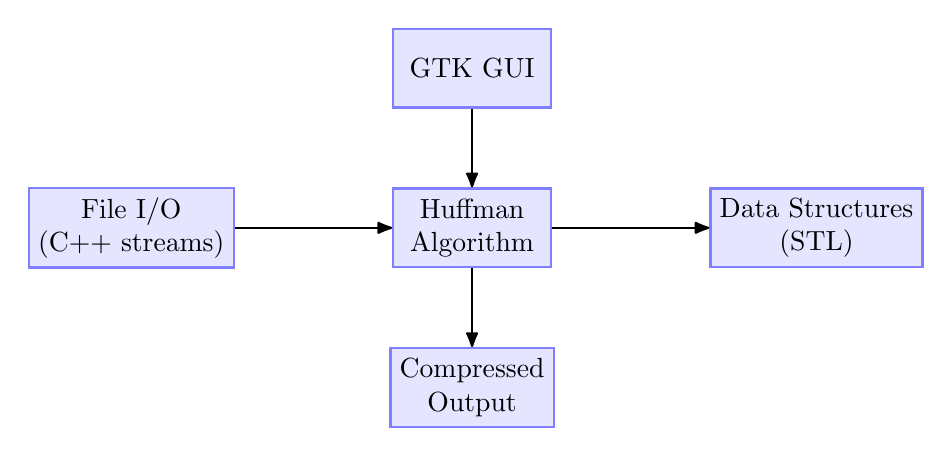
\begin{tikzpicture}[
        node distance=1cm and 2cm,
        box/.style={rectangle, draw=blue!50, fill=blue!10, thick, 
                   minimum height=1cm, minimum width=2cm, align=center},
        arrow/.style={-{Latex[round]}, thick}
    ]
    
    \node[box] (gui) {GTK GUI};
    \node[box, below=of gui] (huffman) {Huffman\\Algorithm};
    \node[box, left=of huffman] (files) {File I/O\\(C++ streams)};
    \node[box, right=of huffman] (data) {Data Structures\\(STL)};
    \node[box, below=of huffman] (output) {Compressed\\Output};
    
    \draw[arrow] (gui) -- (huffman);
    \draw[arrow] (files) -- (huffman);
    \draw[arrow] (huffman) -- (data);
    \draw[arrow] (huffman) -- (output);
    
    \end{tikzpicture}
    \end{center}
\end{frame}

\begin{frame}{Fluxo de Dados}
    \begin{enumerate}
        \item \textbf{Interface GTK} recebe seleção de arquivo
        \item \textbf{C++ File I/O} lê o arquivo original
        \item \textbf{Análise de Frequência} usando \texttt{std::vector<int>}
        \item \textbf{Construção da Árvore} usando \texttt{std::priority\_queue}
        \item \textbf{Geração de Códigos} usando \texttt{std::map}
        \item \textbf{Codificação} com \texttt{BitBuffer} customizado
        \item \textbf{Salvamento} do arquivo comprimido
    \end{enumerate}
\end{frame}

\section{Implementação Real do Projeto GKompress}
\begin{frame}{Arquitetura do Projeto}
    \begin{block}{Estrutura do Código}
        \begin{itemize}
            \item \textbf{Herança}: Classe base \texttt{Huffman} com especializações
            \item \textbf{Polimorfismo}: \texttt{HuffmanTXT}, \texttt{HuffmanBMP}, \texttt{HuffmanWAV}
            \item \textbf{Templates}: Uso de \texttt{std::array}, \texttt{std::vector}, \texttt{std::map}
            \item \textbf{RAII}: Gerenciamento automático de recursos
        \end{itemize}
    \end{block}
    \begin{block}{Padrões de Design}
        \begin{itemize}
            \item \textbf{Strategy Pattern}: Diferentes algoritmos de compressão
            \item \textbf{Template Method}: Fluxo comum de compressão/descompressão
            \item \textbf{Factory Pattern}: Criação de instâncias por tipo de arquivo
        \end{itemize}
    \end{block}
\end{frame}

\begin{frame}[fragile]{Estruturas de Dados Personalizadas - Huffman}
    \begin{lstlisting}[style=CStyle, caption=Estrutura Node personalizada do projeto]
struct Node {
    uint8_t byte;           // Simbolo (para folhas)
    uint32_t duplicates;    // Frequencia do simbolo
    Node* left;            // Filho esquerdo
    Node* right;           // Filho direito
    Node* next;            // Para lista ligada (min-heap manual)
    
    Node(uint8_t b, uint32_t dup) : 
        byte(b), duplicates(dup), 
        left(nullptr), right(nullptr), next(nullptr) {}
        
    int is_leaf() {
        return (left == nullptr && right == nullptr) ? 1 : 0;
    }
};
    \end{lstlisting}
\end{frame}

\begin{frame}[fragile]{Lista Ligada Ordenada - Min-Heap Manual}
    \begin{lstlisting}[style=CStyle, caption=Implementação de lista ordenada para construção da árvore]
class List {
public:
    Node* front = nullptr;
    uint32_t size = 0;
    
    // Insere no mantendo ordem crescente por frequencia
    void insert_sorted(Node* node) {
        if(front == nullptr) {
            front = node;
        } else if(node->duplicates < front->duplicates) {
            node->next = front;
            front = node;
        } else {
            Node* aux = front;
            while(aux->next && aux->next->duplicates < node->duplicates)
                aux = aux->next;
            node->next = aux->next;
            aux->next = node;
        }
        size++;
    }
    
    Node* remove_front() {
        Node* remove = nullptr;
        if(front != nullptr) {
            remove = front;
            front = remove->next;
            remove->next = nullptr;
            size--;
        }
        return remove;
    }
};
    \end{lstlisting}
\end{frame}

\begin{frame}[fragile]{Construção da Árvore de Huffman}
    \begin{lstlisting}[style=CStyle, caption=Algoritmo de construção da árvore]
void HuffmanTree::build(List& list) {
    Node *first_removed, *second_removed, *new_node;
    
    // Repete ate restar apenas um no (raiz)
    while(list.size > 1) {
        // Remove os dois nos com menor frequencia
        first_removed = list.remove_front();
        second_removed = list.remove_front();
        
        // Cria novo no interno
        new_node = new Node('*', 
            first_removed->duplicates + second_removed->duplicates);
        new_node->left = first_removed;
        new_node->right = second_removed;
        new_node->next = nullptr;
        
        // Reinsere na lista ordenada
        list.insert_sorted(new_node);
    }
    root = list.front;
}
    \end{lstlisting}
\end{frame}

\begin{frame}[fragile]{Compressão BMP - Parte 1}
    \begin{lstlisting}[style=CStyle, caption=Leitura e análise de frequências]
void HuffmanBMP::compress(int option) {
    // Le arquivo BMP com headers
    bmp_file.read(filepath.c_str());
    
    // Conta frequencias apenas dos dados de imagem
    count_duplicates(bmp_file.data, bmp_file.data_size);
    
    // Constroi arvore e dicionario
    list.fill(duplicates);
    tree.build(list);
    size_t max_columns = tree.height();
    dictionary.build(max_columns);
    dictionary.fill(tree.root, "", max_columns, option);

    // Codifica apenas os dados, preserva headers
    char* code = encode(bmp_file.data, bmp_file.data_size);
    internal_compress(option, code, write_bmp_header, &bmp_file);
}
    \end{lstlisting}
\end{frame}

\begin{frame}[fragile]{Compressão BMP - Parte 2}
    \begin{lstlisting}[style=CStyle, caption=Codificação e salvamento]
// Funcao callback para escrever headers BMP
static void write_bmp_header(FILE* file, void* image_file) {
    bmp* bmp_ptr = static_cast<bmp*>(image_file);
    fwrite(&bmp_ptr->header, sizeof(bmp_ptr->header), 1, file);
    fwrite(&bmp_ptr->info_header, sizeof(bmp_ptr->info_header), 1, file);
    if(bmp_ptr->has_color_table()) {
        fwrite(bmp_ptr->color_table, 
               bmp_ptr->get_color_table_size(), 1, file);
    }
}
    \end{lstlisting}
\end{frame}

\begin{frame}{Estruturas de Dados e Performance}
    \begin{block}{Complexidade Temporal}
        \begin{itemize}
            \item Análise de frequência: O(n)
            \item Construção da árvore: O(k log k) onde k = símbolos únicos
            \item Codificação: O(n)
            \item \textbf{Total: O(n + k log k)}
        \end{itemize}
    \end{block}
    \begin{block}{Complexidade Espacial}
        \begin{itemize}
            \item Array de frequências: O(1) - tamanho fixo
            \item Árvore de Huffman: O(k)
            \item Mapa de códigos: O(k)
            \item \textbf{Total: O(k)}
        \end{itemize}
    \end{block}
\end{frame}

\begin{frame}{Vantagens das Estruturas Escolhidas}
    \begin{block}{STL - Standard Template Library}
        \begin{itemize}
            \item \textbf{priority\_queue}: Heap otimizado para construção da árvore
            \item \textbf{map}: Busca eficiente de códigos O(log n)
            \item \textbf{vector}: Arrays dinâmicos com acesso O(1)
        \end{itemize}
    \end{block}
    \begin{block}{C++ vs Outras Linguagens}
        \begin{itemize}
            \item \textbf{Performance}: Controle total sobre memória
            \item \textbf{Portabilidade}: Código executável nativo
            \item \textbf{Integração}: Compatibilidade com GTK
        \end{itemize}
    \end{block}
\end{frame}

\section{Conclusões}
\begin{frame}{Lições Aprendidas}
    \begin{block}{Estruturas de Dados}
        \begin{itemize}
            \item Escolha adequada impacta diretamente na performance
            \item STL oferece implementações otimizadas
            \item Customização necessária para casos específicos (BitBuffer)
        \end{itemize}
    \end{block}
    \begin{block}{Ferramentas}
        \begin{itemize}
            \item C++ ideal para algoritmos de baixo nível
            \item GTK proporciona interface profissional
            \item Integração entre ferramentas é crucial
        \end{itemize}
    \end{block}
\end{frame}
\end{document}
